\documentclass[11pt]{article}

\usepackage[margin=1in]{geometry}
\geometry{
  a4paper,         % or letterpaper
  textwidth=16cm,  % llncs has 12.2cm
  textheight=24cm, % llncs has 19.3cm
  heightrounded,   % integer number of lines
  hratio=1:1,      % horizontally centered
  vratio=2:3,      % not vertically centered
}

\renewcommand\labelitemi{*}

% Packages
% ------------------
% \usepackage{tkz-euclide}
\usepackage{tikz} % for drawing diagrams
\usepackage{bm} % bold mode
%% \usepackage{color}
\usepackage{hyperref}

% setup style of tikzlibrary elements
% ------------------------------------
\usetikzlibrary{arrows}
\usetikzlibrary{quotes,angles}
\usetikzlibrary{positioning}
\usetikzlibrary{plotmarks}
\usetikzlibrary{shapes.geometric, arrows}

% setup style of tikzlibrary elements
% ------------------------------------
\tikzstyle{block} = [rectangle, minimum width=2.5cm, minimum height=1cm, text centered, text width=2.7cm, draw=black, fill=white]
\tikzstyle{redblock} = [rectangle, thick, minimum width=2.5cm, minimum height=1cm, text centered, text width=2.7cm, draw=red, fill=white]
\tikzstyle{wideblock} = [rectangle, minimum width=2.5cm, minimum height=1cm, text centered, text width=5cm, draw=black, fill=white]
\tikzstyle{tallblock} = [rectangle, minimum width=1.9cm, minimum height=2cm, text centered, text width=1.9cm, draw=black, fill=white]
\tikzstyle{inputblock} = [rectangle, minimum width=1.7cm, minimum height=5cm, text centered, text width=1.7cm, draw=black, fill=white]
\tikzstyle{sumation} = [circle, minimum width=0.2cm, minimum height=0.5cm, text centered, text width=0.4cm, draw=black, fill=white]

\tikzstyle{startstop} = [rectangle, rounded corners, minimum width=3cm, minimum height=1cm, text centered, draw=black, fill=white]
\tikzstyle{io} = [trapezium, trapezium left angle=70, trapezium right angle=110, minimum width=3cm, minimum height=1cm, text centered, draw=black, fill=white]
\tikzstyle{process} = [rectangle, minimum width=4cm, minimum height=1cm, text centered, text width=4cm, draw=black, fill=white]
\tikzstyle{decision} = [diamond, minimum width=3cm, minimum height=1cm, text centered, draw=black, fill=white]
\tikzstyle{arrow} = [->,>=stealth] % can add "thick" to make it bold
\tikzset{radiation/.style={{decorate,decoration={expanding waves,angle=90,segment length=4pt}}}}

% new commands
% ------------------
\definecolor{light-gray}{gray}{0.95}
\newcommand{\code}[1]{\colorbox{light-gray}{\texttt{#1}}}


\begin{document}

% {\Huge Project Description} % optional

% Header of paper
% NOTE: The \maketitle command MUST come AFTER the \begin{document} command!
% ---------------------
\title{TikZ Playground}
\author{
  Author: Sergio Garc\'{i}a-Vergara \\
  \small{https://www.sergiogarciavergara.com}
}

\maketitle

%@@@@@@@@@@@@@@@@@@@@@@@@@@@@@@@@@@@@@@@@@@@@@@@@@@

% Abstract
% ---------------------
\begin{abstract}

  This sample tex file is intended to be used together with the tutorials on the
  TikZ package described in Sergio's website
  (\href{https://www.sergiogarciavergara.com/block-diagrams-in-latex/}{https://www.sergiogarciavergara.com/block-diagrams-in-latex/}). The
  tutorials describe step-by-step how to construct the diagrams and flowcharts
  shown in this document.

\end{abstract}


% @@@@@@@@@@@@@@@@@@@@@@@@@@@@@@@@@@@@@@@@@@@@@@@@@@

\section{Block Diagrams}
% ---------------------------

Let's look at a simple Feedback Diagram. Consider the transfer function for a
noise-free physical linear system (\ref{eq:linear_system_trans_fun}):

\begin{equation}\label{eq:linear_system_trans_fun}
Y(s) = \frac{C(s)}{R(s)} = \frac{KG(s)}{1 + KG(s)H(s)}
\end{equation}

\noindent
where $C(s)$ and $R(s)$ are the output and input of the system,
respectively. It's corresponding block diagram is represented by Figure
\ref{fig:liner_system_diagram}.

\begin{figure}[h]
\begin{center}
\begin{tikzpicture}[auto, node distance=2.7cm, >=latex']

  % We start by placing the blocks
  \node (input) [circle] {R(s)};

  \node (sum) [sumation, right of=input, xshift=-0.4cm] {};
  \node (plus_sign) [above of=sum, xshift=-0.6cm, yshift=-2.4cm] {+};
  \node (minus_sign) [below of=sum, xshift=-0.4cm, yshift=2.1cm] {-};
  \node (kgs) [block, right of=sum, xshift=0.45cm] {KG(s)};
  \node (hs) [block, below of=kgs, yshift=0.7cm] {H(s)};
  \node (output) [circle, right of=kgs, xshift=1.2cm] {C(s)};

  % Draw the connections between blocks
  \draw [arrow] (input) -- node[anchor=north] {} (sum);
  \draw [arrow] (sum) -- node[anchor=north] {} (kgs);
  \draw [arrow] (kgs) -- node[anchor=north] {} (output);
  \draw [arrow] (kgs.0) -| ++(1cm,0cm) |- node[anchor=north] {} (hs.0);
  \draw [arrow] (hs.180) -| node[anchor=north] {} (sum.270);
  % \draw [arrow] (main_box.0) -| ++(-1cm,0) |- node[anchor=south, xshift=0.4cm] {tracks} (level1.0);

\end{tikzpicture}
\end{center}
 \caption{Block diagram of a noise-free linear system.}
\label{fig:liner_system_diagram}
\end{figure}


\newpage

%@@@@@@@@@@@@@@@@@@@@@@@@@@@@@@@@@@@@@@@@@@@@@@@@@@

\section{Flowchart}
% ---------------------------

The sterile processing departments in hospitals are responsible for processing
the surgical instruments and making sure that they're ready before every
surgery. Sometimes, instruments are missing at the time of preparing a surgical
tray. The following flowchart describes how technicians handle these
situations:

\begin{figure}[h]
\begin{center}
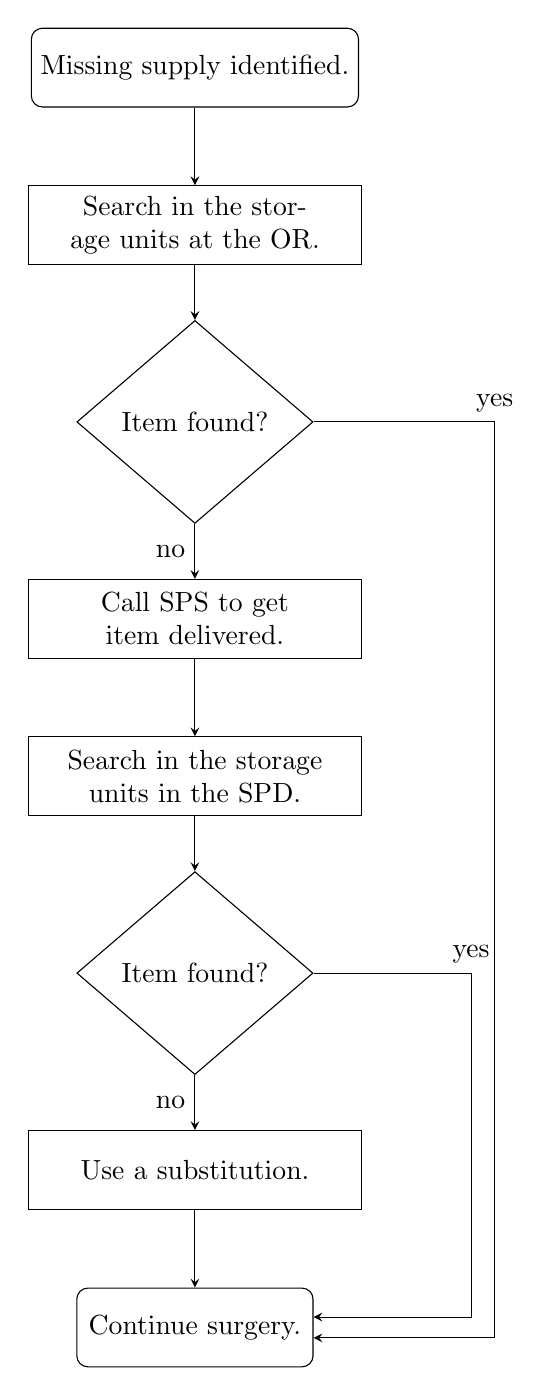
\begin{tikzpicture}[auto, node distance=2cm, >=latex']

  % We start by placing the blocks
  \node (start) [startstop] {Missing supply identified.};
  \node (searchor) [process, below of=start] {Search in the storage units at the OR.};
  \node (foundor) [decision, below of=searchor, yshift=-0.5cm] {Item found?};
  \node (callsps) [process, below of=foundor, yshift=-0.5cm] {Call SPS to get item delivered.};
  \node (searchsps) [process, below of=callsps] {Search in the storage units in the SPD.};
  \node (foundsps) [decision, below of=searchsps, yshift=-0.5cm] {Item found?};
  \node (substitution) [process, below of=foundsps, yshift=-0.5cm] {Use a substitution.};

  \node (continue) [startstop, below of=substitution] {Continue surgery.};

  % draw connections between nodes
  \draw [arrow] (start) -- (searchor);
  \draw [arrow] (searchor) -- (foundor);
  \draw [arrow] (foundor) -- node[anchor=east] {no} (callsps);
  \draw [arrow] (foundor.0) -| node[anchor=south] {yes} ++(2.3cm,0) |- (continue.355);
  \draw [arrow] (callsps) -- (searchsps);
  \draw [arrow] (searchsps) -- (foundsps);
  \draw [arrow] (foundsps) -- node[anchor=east] {no} (substitution);
  \draw [arrow] (foundsps.0) -| node[anchor=south] {yes} ++(2cm,0) |- (continue.5);
  \draw [arrow] (substitution) -- (continue);

\end{tikzpicture}
\end{center}
\caption{Workflow for what happens when someone notices that there is a missing
  instrument or disposable at the OR.}
\label{fig:missing_instrument_workflow}
\end{figure}

\newpage

%@@@@@@@@@@@@@@@@@@@@@@@@@@@@@@@@@@@@@@@@@@@@@@@@@@

\section{General Drawings}
% ---------------------------


% @@@@@@@@@@@@@@@@@@@@@@@@@@@@@@@@@@@@@@@@@@@@@@@@@@

% \newpage
% \bibliographystyle{ieeetr}
% \bibliography{references}

\end{document}

%%% Local Variables:
%%% mode: latex
%%% TeX-master: t
%%% End:
